% !TEX root = ../main.tex
\subsection{RG-E Experiment} \label{ssec::rgeexperiment}
    The Run Group E (RG-E) experiment aims to measure the hadronic multiplicity ratio between different nuclei and deuterium.
    To do this, a double-target system is being built to be used in Hall B.
    The system will allow a precise comparison of a deuterium target and heavy solid targets, like carbon, aluminium, copper, tin, lead, etc.
    The experiment aims to further the understanding of hadronisation in the nuclear medium, colour transparency, and nuclear short-range correlations.

    During data acquisition, the cryo-target (deuterium) and a solid target will be exposed to the electron beam simultaneously.
    To minimise acceptance correction difference between targets, we aim to keep the distance between them as low as possible -- as long as we can differentiate between the targets in reconstruction.
    Part of this thesis' work involves improving offline reconstruction before the experiment to reduce this distance, which can be read in chapter \ref{sec::fmtalignmentandreconstruction}.
    
    Positioning both targets in the beam simultaneously allows us to cancel time-dependent systematic effects o increase the precision of final results.
    These include effects such as drifting gains and inefficient detector channels in the measurement of ratio-like observables.
    Then, since the target system will be in a vacuum, the switching between solid targets will need to be performed remotely.
    Additionally, it needs to be done as quickly as possible, to maximise the beam time of the experiment.

    The double target system will be able to switch between up to five different solid targets.
    The previous EG2 experiment performed on the former CLAS showed that the design of the double target system has significant advantages to reduce the systemic uncertainties \cite{hakobyan2008}.
    The principle of the target system is to have the solid targets installed on a carbon fibre band which slides on torlon rails.
    The band is moved by a piezo-motor, which -- like all other chosen materials -- is insensitive to magnetic fields.
    The design proposed can be seen in figure \ref{fig::double_target}.
    
    \begin{figure}[b!]
        \centering\frame{
        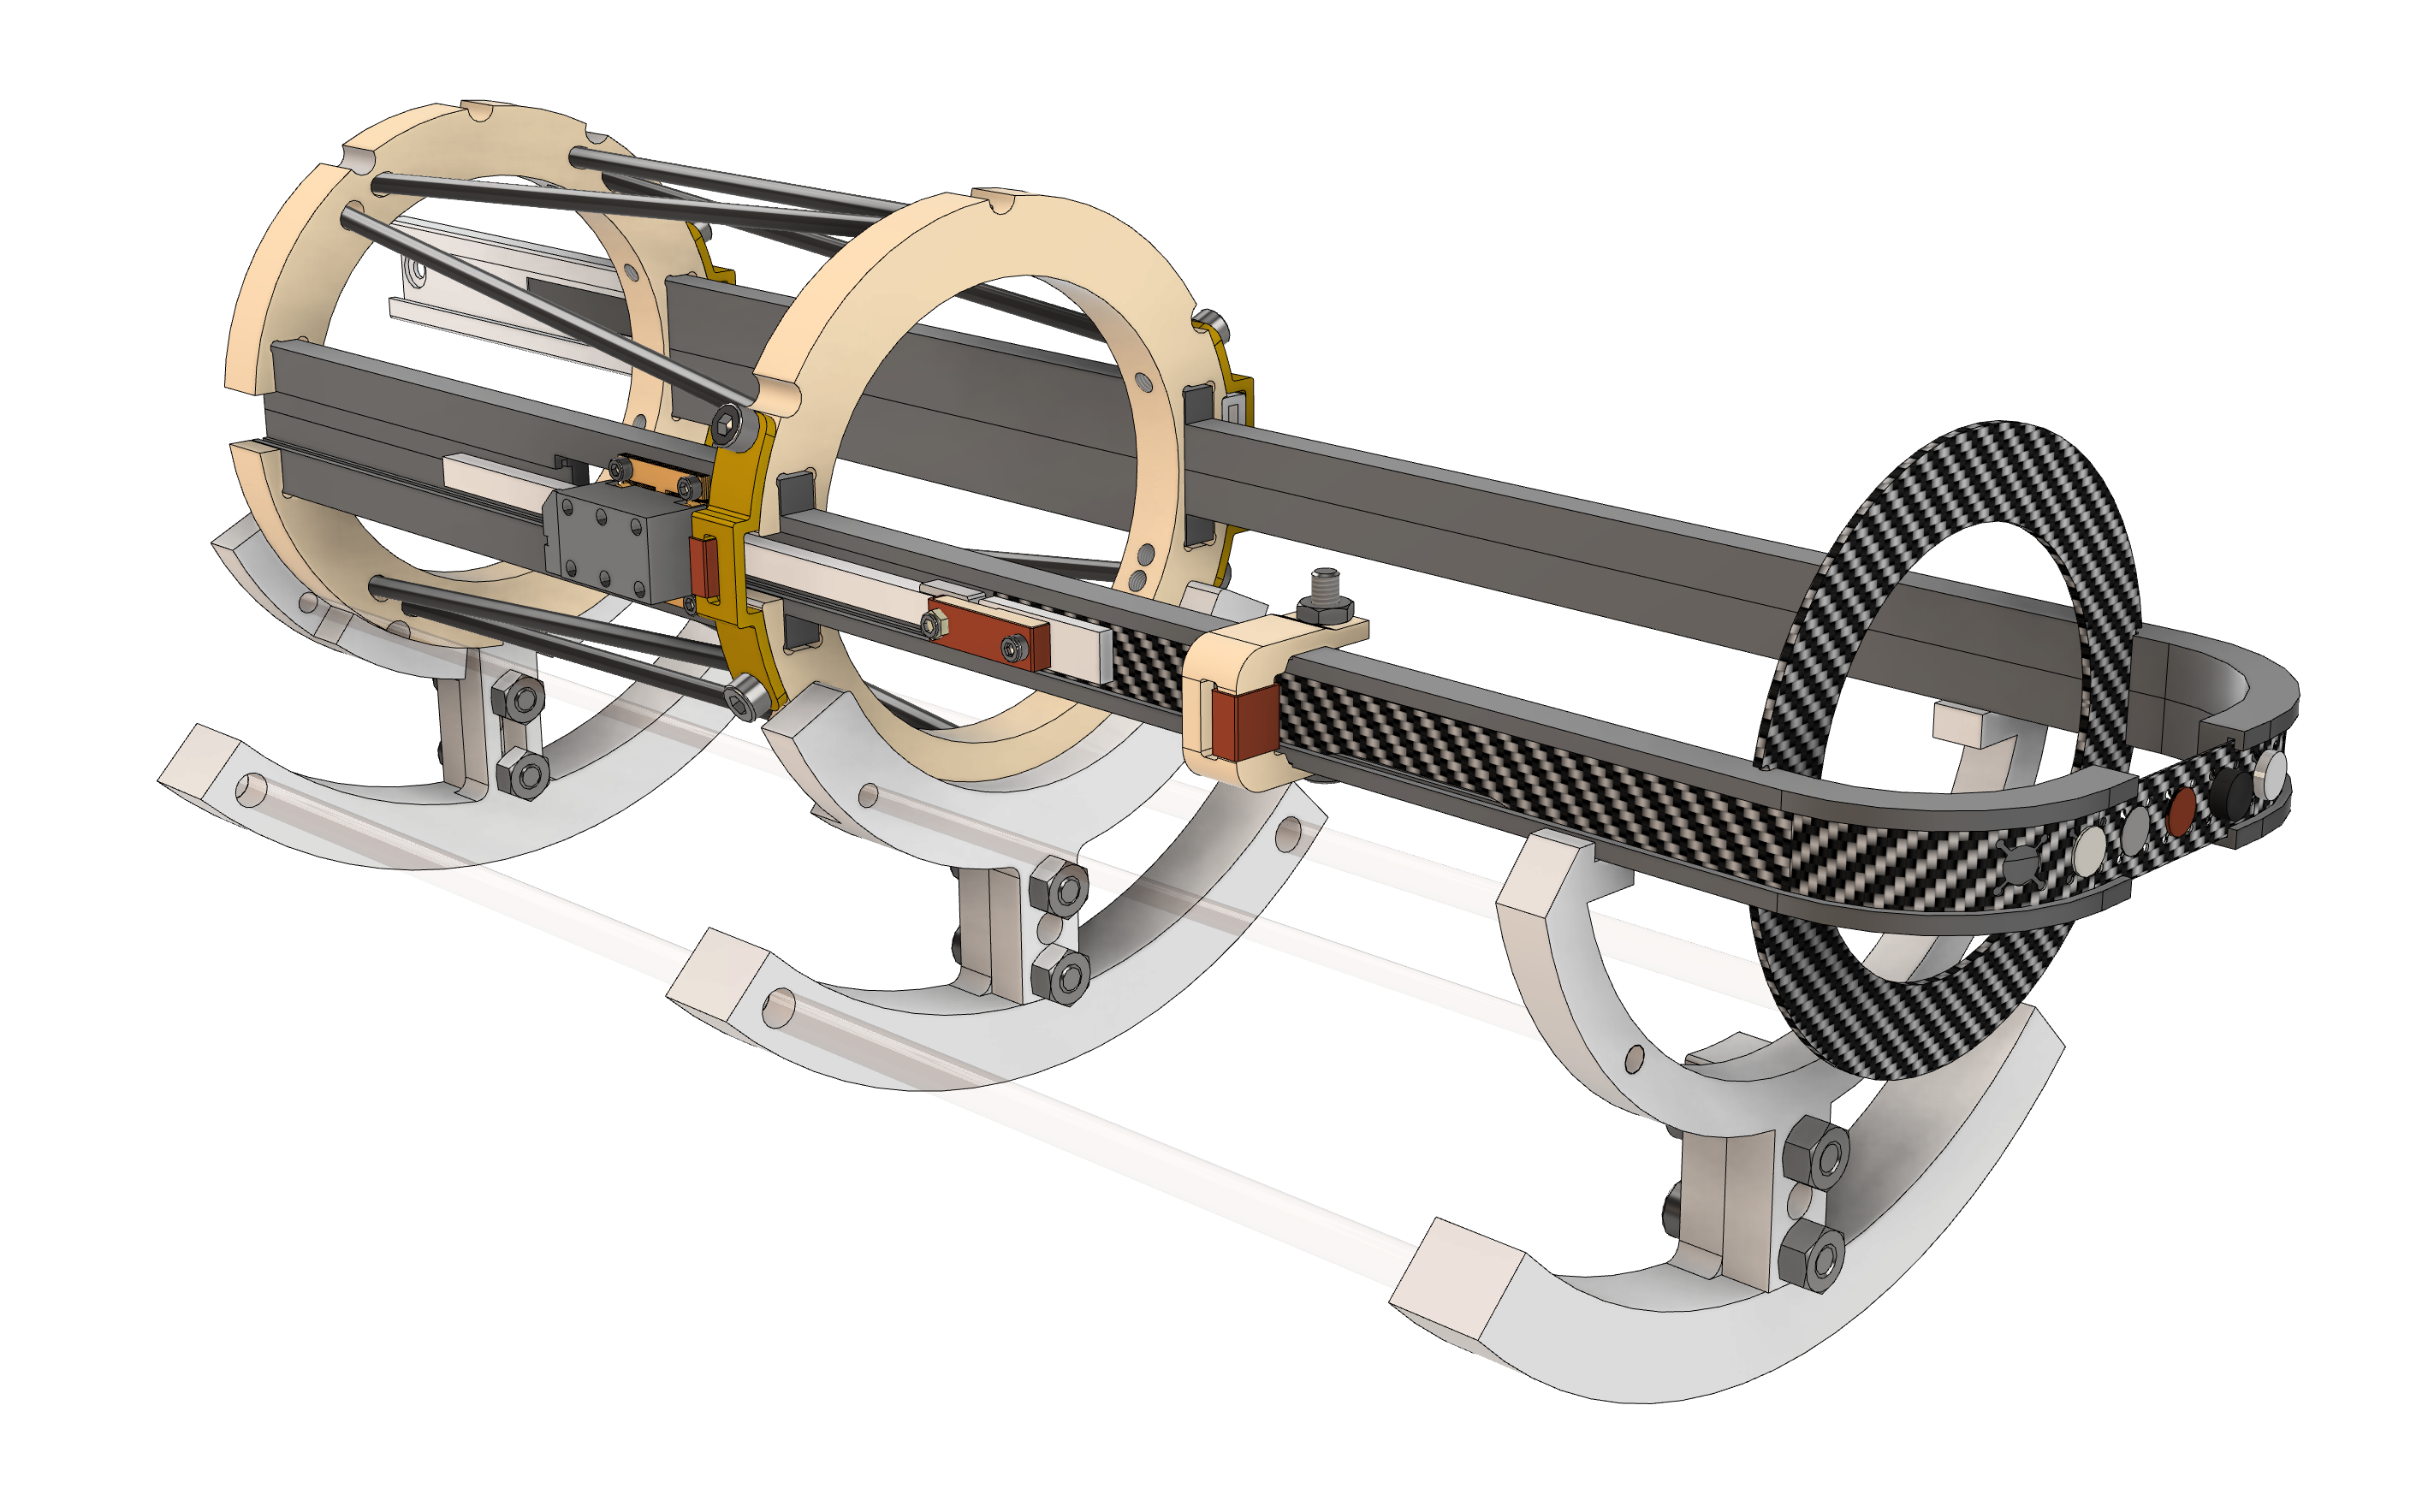
\includegraphics[width=\textwidth]{11experiment/img/30double_target.png}}
        \caption[Double-target system.]{Double-target system CAD render.}
        \label{fig::double_target}
    \end{figure}

    To ensure the adequate operation of the target, several tests were performed.
    These include movement under vacuum and high magnetic field, radiation hardness of the selected materials, and heat removal tests which secure that target remain far below melting point.
    
    % !TEX root = ../main.tex
\subsubsection{Slow Control System} \label{sssec::slowcontrolsystem}
% --+ What is slow control +----------------------------------------------------
    A modern experimental physics experiment usually involves many of moving parts and complex components that need constant monitoring and calibration.
    This is in addition to the constant data taking necessary.
    The process of automating this task is made via slow controls systems.
    These systems usually integrate a whole detector and experiment into one complex interface, allowing for easy access and maintenance.

% --+ What is EPICS +-----------------------------------------------------------
    The standard framework to do this in the context of HEP is the Experimental Physics and Industrial Control System (EPICS).
    EPICS was developed in the Los Alamos National laboratory (ANL) to provide data acquisition and control to this type of experiments.
    The framework provides a distributed process control that includes software communication, functional subsystems for data acquisition, supervisory control, closed loop control, channel archiving, and alarm management \cite{dalesio1991}.
    Like many HEP experiments, CLAS12's slow control system is based on EPICS \cite{boyarinov2020}.

% --+ EPICS installation on raspi +---------------------------------------------
    To allow the integration of the RG-E target on the CLAS12 slow controls system, an EPICS support module and Input / Output Controller (IOC) was developed by the author.
    This module wasn't made from scratch, as the motor developers made a generic support module for Galil motors \cite{farnswort2009}.
    This system proved to support all that was necessary for the movement of the RG-E target system, only requiring the removal of unnecessary features and the addition of database variables relevant to the experiment.
    % NOTE. This chapter doesn't involve the integration of thermocouples, as that is left as future work.

    The Process Variables (PVs) added to the EPICS module are listed, along with a short description of each.
    Each of these can be viewed and edited at the user-defined records database, which is at

    \begin{center}
        \texttt{\$EPICS\_BASE/support/galil/3-6/db/galil\_userdef\_records.template}.
    \end{center}

    \paragraph{Analog Input (\texttt{ai})}
        The normal use for this record type is to obtain an analog value from hardware and then convert it to engineering units \cite{stanley1998}.
        The record can also be used to write constants to be read from the database, such that they can be changed in runtime.

        \subparagraph{\texttt{DMC01:A\_curr\_pos}.}
            Current position of the band.
            Displayed at the GUI and used for internal calculations.

        \subparagraph{\texttt{DMC01:A\_home}.}
            Position of the home.
            Displayed at the GUI and used for calculations.

        \subparagraph{\texttt{DMC01:A\_pos\#}.}
            \# is a number from 1 to 7.
            Positions of each of the seven targets.
            Displayed at the GUI and used for calculations.

        \subparagraph{\texttt{DMC01:A\_lowlimit}.}
            Position of the low limit.
            If \texttt{DMC01:A\_curr\_pos} is lesser than this value, a major alarm is fired.

        \subparagraph{\texttt{DMC01:A\_highlimit}.}
            Position of the high limit.
            If \texttt{DMC01:A\_curr\_pos} is greater than this value, a major alarm is fired.

        \subparagraph{\texttt{DMC01:A\_tolerance}.}
            Equivalence tolerance for the position of each target and the position of the band.
            It defines a valid range around the target position.

        \subparagraph{\texttt{DMC01:COMMERR\_STATUS}.}
            Variable that is true when there's a communication error with the controller and false otherwise.
            Used for triggering a communication alarm.

        \subparagraph{\texttt{IOC01:SR\_i\_am\_alive}.}
            Variable that is true when the IOC is up and running, false otherwise.
            Used for triggering a communication alarm.

    \paragraph{Analog Output (\texttt{ao})}
        The normal use for this record type is to output values to digital-analog converters.
        The desired output can be controlled by either an operator or a state program, or it can be fetched from another record \cite{stanley1998}.

        \subparagraph{\texttt{DMC01:A\_go\_home}.}
            Command to move the band to the home position, as defined in \texttt{DMC01:A\_home}.

        \subparagraph{\texttt{DMC01:A\_go\_pos\#}.}
            Command to move the band to the position of target \#, as defined in \texttt{DMC01:A\_pos\#}.

    \paragraph{Calculation (\texttt{calc})}
        The calculation or ``Calc'' record is used to perform algebraic, relational, and logical operations on values retrieved from other records.
        The result of its operations can then be accessed by another record so that it can be used \cite{stanley1998}.
        In the context of the RG-E target, each calculation returns a number from 0 to 11.
        This number represent the state the target is in, and is later used by a Select PV.

        \subparagraph{\texttt{DMC01:A\_at\_pos\#}.}
            Calculation that checks if the band position is equal to that of target \# in \texttt{DMC01:A\_pos\#}, within the tolerance margin \texttt{DMC01:A\_tolerance}.
            If it is, it returns \#.
            Otherwise, it returns 0.

        \subparagraph{\texttt{DMC01:A\_at\_home}.}
            Calculation that checks if the band position is equal to the home position in \texttt{DMC01:A\_home}, within the tolerance margin defined by the tolerance.
            If it is, it returns 8.
            Otherwise, it returns 0.

        \subparagraph{\texttt{DMC01:A\_moving}.}
            Calculation that checks if the target is moving by checking the motor PV \texttt{DMC01:A.MOVN}.
            If it is, it returns 9.
            Otherwise, it returns 0.

        \subparagraph{\texttt{DMC01:A\_at\_lowlimit}.}
            Calculation that checks if the band position is lesser than the low limit \texttt{DMC01:A\_lowlimit}.
            If it is, it returns 10.
            Otherwise, it returns 0.

        \subparagraph{\texttt{DMC01:A\_at\_highlimit}.}
            Calculation that checks if the band position is greater than the high limit \texttt{DMC01:A\_highlimit}.
            If it is, it returns 11.
            Otherwise, it returns 0.

    \paragraph{Select (\texttt{sel})}
        The select record computes a value based on input obtained from up to 12 locations.
        By default, it is equal to the highest value among its input PVs \cite{stanley1998}.

        \subparagraph{\texttt{DMC01:A\_sel\_tgttype}.}
            This record returns the highest value between the previously defined calculations.
            Thus, it associates the values returned to a state of the target.
            By convention, this PV assumes that \emph{no more than one \texttt{calc} is greater than 0}.
            This assumptions holds as long as \texttt{DMC01:A\_tolerance} is not set higher than half the distance between targets and between the targets and the lower and higher limits.

    \paragraph{Multi-Bit Binary Input (\texttt{mbbi})}
        The normal use for the multi-bit binary input record is to read multiple bit inputs from hardware.
        The binary value represents a state from a range of up to 16 states.
        The multi-bit input record interfaces with devices that use more than one bit \cite{stanley1998}.

        \subparagraph{\texttt{DMC01:A\_tgttype}.}
            This \texttt{mbbi} encodes the output of \texttt{DMC01:A\_sel\_tgttype} to a string and alarm level.
            The encoding is specified in table \ref{tab::tgttypespv}.

    \begin{table}[b!]
        \caption{Names and alarm levels for the different values of the PV \texttt{DMC01:A\_tgttype}.}

        \begin{center}
            \begin{tabularx}{220pt}{lll}
                \hline
                \textbf{Value} & \textbf{Name} & \textbf{Alarm Severity} \\
                \hline
                 0             & Not Moving    & Major                   \\
                 1             & Target 1      & No alarm                \\
                 2             & Target 2      & No alarm                \\
                 3             & Target 3      & No alarm                \\
                 4             & Target 4      & No alarm                \\
                 5             & Target 5      & No alarm                \\
                 6             & Target 6      & No alarm                \\
                 7             & Target 7      & No alarm                \\
                 8             & Home          & No alarm                \\
                 9             & Moving        & Minor                   \\
                10             & Low Limit     & Major                   \\
                11             & High Limit    & Major                   \\
                \hline
            \end{tabularx}
        \end{center}
        \label{tab::tgttypespv}
    \end{table}

    The RG-E IOC, along with the complete set of EPICS support modules necessary to run it, can be found at

    \begin{center}
        \hyperlink{https://github.com/bleaktwig/rge-epics-support}{\texttt{https://github.com/bleaktwig/rge-epics-support}}.
    \end{center}

    \paragraph{CS-Studio}
        The Graphical User Interface (GUI) of CLAS12 EPICS is based on the Control System Studio (CS-Studio) toolkit.
        CS-Studio is used to monitor and operate large scale control systems, and is based on the eclipse Rich Client Platform (RCP) framework \cite{kasemir2007}.
        In order to integrate the RG-E target system into CLAS12 EPICS, a CS-Studio screen needed to be developed.

        The set of requirements the screen needed to fulfil are listed.
        These requirements are based both on the specifications of the physics experiments and the needs of the electronics team behind the target.
        \begin{itemize}
            \item
                Buttons to move the target band to the targets and a home location.
            \item
                A Button to stop the target band in case of emergency.
            \item
                A status check on the position of the target band.
            \item
                Alarm handling for the case when the band moves beyond low and high limits.
            \item
                Alarm handling for the IOC and communication problems.
        \end{itemize}
        These requirements were implemented in the screen, which can be seen in figure \ref{fig::rge_motorx}.
        In addition to the buttons, text displays show the position of each target in the band.
        LED displays to the right of these light up green when the band position matches the target position, within a tolerance defined in the database.
        Finally, four LED displays are laid in to the right of the two IOC statuses and the low and high limits.
        These show alarm conditions, acting in tandem with the CLAS12 Slow Control alarm system to alert the user of a problem.

        \begin{figure}[t!]
            \centering\frame{
            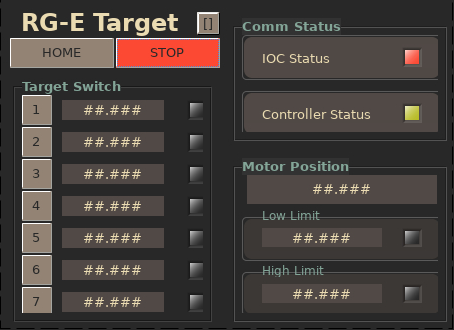
\includegraphics[]{11experiment/img/31motorx_rge.png}}
            \caption[RG-E CS-Studio main screen]{RG-E CS-Studio main screen. The HOME and A, B, C, etc buttons move the target strip to the corresponding location, the STOP button is an emergency, instant stop of the target system, and the Motor Screens button allows the user to open additional motor screens.}
            \label{fig::rge_motorx}
        \end{figure}

        In addition to this screen, other screens can be accessed through the Motor Screens menu button.
        These screens are part of the motor EPICS support module, and are left in case any debugging is necessary.
        These screens include a screen that allows for manual motor movement, a motor setup screen, a direct Command Line Interface (CLI) with the motor, and an amplifier configuration screen.
        All of these screens were developed by the Galil EPICS team \cite{farnswort2009}.

        For the user's comfort, the GUI was coloured using the Gruvbox colour palette.
        This palette is designed to keep colours easily distinguishable, contrast enough, while being pleasing for the eyes.
        Gruvbox can be found on GitHub at

        \begin{center}
            \hyperlink{https://github.com/morhetz/gruvbox}{\texttt{https://github.com/morhetz/gruvbox}}.
        \end{center}

    \paragraph{Alarm System}
        To secure the good functioning of the CLAS12 detector, all its subsystems controlled via EPICS contain PVs that specify alarm conditions.
        A centralised alarm system displays these alarms, together with their severity, associated subsystems, and pre-written guidance on how to react to them.
        For each experiment with a non-trivial target done in Hall B, the target system requires its own list of alarms.

        For the RG-E target, the set of alarms implemented and their related PVs are listed in table \ref{tab::alarmspv}.

        \begin{table}[b!]
            \caption{Alarm names, triggers, and severities for the RG-E target slow control system.}

            \begin{center}
                \begin{tabularx}{360pt}{llX}
                    \hline
                    \textbf{Name}          & \textbf{Trigger}                     & \textbf{Severity} \\
                    \hline
                    Band is not moving     & \texttt{DMC01:A\_tgttype}       =  0 & Major             \\
                    Band is moving         & \texttt{DMC01:A\_tgttype}       =  9 & Minor             \\
                    Band beyond low limit  & \texttt{DMC01:A\_tgttype}       = 10 & Major             \\
                    Band beyond high limit & \texttt{DMC01:A\_tgttype}       = 11 & Major             \\
                    Controller comm. error & \texttt{DMC01:COMMERR\_STATUS}  =  1 & Major             \\
                    IOC comm. error        & \texttt{IOC01:SR\_i\_am\_alive} =  0 & Major             \\
                    \hline
                \end{tabularx}
                \label{tab::alarmspv}
            \end{center}
        \end{table}

